
\documentclass[14pt]{beamer}

\usepackage[T1]{fontenc}

\setbeamertemplate{navigation symbols}{}
\useoutertheme{infolines}
\useinnertheme{circles}
\usecolortheme{fly}


\usepackage{eulervm}
\usefonttheme[onlymath]{serif}

\makeatother
\setbeamertemplate{footline}
{
  \leavevmode%
  \hbox{%
  \begin{beamercolorbox}[wd=.4\paperwidth,ht=2.25ex,dp=1ex,center]{author in head/foot}%
    \usebeamerfont{author in head/foot}\insertshortauthor
  \end{beamercolorbox}%
  \begin{beamercolorbox}[wd=.6\paperwidth,ht=2.25ex,dp=1ex,center]{title in head/foot}%
    \usebeamerfont{title in head/foot}\insertshorttitle\hspace*{3em}
    \insertframenumber{} / \inserttotalframenumber\hspace*{1ex}
  \end{beamercolorbox}}%
  \vskip0pt%
}

\usepackage{mathtools}

\newcommand{\ttd}{\mathrm{d}}
\newcommand{\ttdx}{\mathrm{d}x}
\newcommand{\ttdt}{\mathrm{d}t}
\newcommand{\ifnonlif}{\quad\Leftrightarrow\quad}

\newcommand{\lam}[2]{{\backslash{#1}\mapsto{#2}}}

\def\clap#1{\hbox to 0pt{\hss#1\hss}}
\def\mathllap{\mathpalette\mathllapinternal}
\def\mathrlap{\mathpalette\mathrlapinternal}
\def\mathclap{\mathpalette\mathclapinternal}
\def\mathllapinternal#1#2{%
\llap{$\mathsurround=0pt#1{#2}$}}
\def\mathrlapinternal#1#2{%
\rlap{$\mathsurround=0pt#1{#2}$}}
\def\mathclapinternal#1#2{%
\clap{$\mathsurround=0pt#1{#2}$}}

\newcommand{\prescripts}[2]{\phantom{{}^{#1}_{#2}}{}^{\mathllap{#1}}_{\mathllap{#2}}}

\newcommand{\lambdaf}[2]{\backslash{#1}\mapsto{#2}}

\newcommand{\identity}{\mathrm{id}}


\newcommand{\casessonst}[2]{\begin{cases} #1 \\ #2 & \mbox{sonst}\end{cases}}
\newcommand{\caseselse}[2]{\begin{cases} #1 \\ #2 & \mbox{else}\end{cases}}

\newcommand{\betterbe}{\overset{!}{=}}
\newcommand{\forceeq}{\overset{!}{=}}
\newcommand{\modeq}[3]{#2\equiv#3\;|\,\mathrm{mod}\,#1\,}

\newcommand{\thus}{{\Rightarrow\quad}}

\newcommand{\ket}[1]{|\, #1 \rangle}
\newcommand{\Ket}[1]{\left| #1 \right\rangle}
\newcommand{\bra}[1]{\langle #1 \,|}
\newcommand{\Bra}[1]{\left\langle #1 \right|}
\newcommand{\braket}[2]{\langle{#1}\,|\,{#2}\rangle}
\newcommand{\braKet}[2]{\left\langle{#1}\Ket{#2}\right.}
\newcommand{\Braket}[2]{\left.\Bra{#1}{#2}\right\rangle}
\newcommand{\braOPket}[3]{\left\langle{#1}\left|{#2}\right|{#3}\right\rangle}
\newcommand{\braopket}[3]{\bra{#1}{#2}\ket{#3}}
\newcommand{\braopKet}[3]{\left\langle{#1}\left|{#2}\Ket{#3}\right.\right.}
\newcommand{\Braopket}[3]{\left.\left.\Bra{#1}{#2}\right|{#3}\right\rangle}

\newcommand{\bbv}[1]{\boldsymbol{#1}}

\newcommand{\ptdiffby}[1]{\frac{\partial}{\partial{#1}}}
\newcommand{\tptdiffby}[1]{\tfrac{\partial}{\partial{#1}}}
\newcommand{\ptntdfby}[2]{\frac{\partial^{#2}}{\partial{#1}^{#2}}}
\newcommand{\tptntdfby}[2]{\tfrac{\partial^{#2}}{\partial{#1}^{#2}}}
\newcommand{\tdyndfh}[3]{\left(\frac{\partial{#1}}{\partial{#2}}\right)_{\!\!#3}}
\newcommand{\ttdyndfh}[3]{(\tfrac{\partial{#1}}{\partial{#2}})_{#3}}


% \usepackage{eulervm}
\DeclareMathAlphabet\mathupit{U}{zeur}{m}{n}

\newcommand{\romanizeXyz}[1]{\IfStrEq{#1}{x}{\mathrm{x}}%
                            {\IfStrEq{#1}{y}{\mathrm{y}}%
                            {\IfStrEq{#1}{z}{\mathrm{z}}%
                            {#1}}}}
\newcommand{\romanizeTxyz}[1]{\IfStrEq{#1}{x}{\mathrm{x}}%
                             {\IfStrEq{#1}{y}{\mathrm{y}}%
                             {\IfStrEq{#1}{z}{\mathrm{z}}%
                             {\IfStrEq{#1}{t}{\mathrm{t}}%
                             {#1}}}}}


\newcommand{\physu}[1]{\mathrm{#1}}

\newcommand{\chinl}[1]{$\mathrm{#1}$ }


%\newcommand{\vnab}{\vec{\nabla}}

\newcommand{\kbar}{\mathrlap{\bar{\,\ }}k}
\newcommand{\kbarT}{\kbar T}

\newcommand{\Angstrom}{\buildrel {_\circ} \over {\mathrm{A}}}

\newcommand{\sqthf}{\frac{1}{\sqrt{2}}}
\newcommand{\tsqthf}{\tfrac{1}{\sqrt{2}}}

\newcommand{\QED}{\begin{flushright}$\square$\end{flushright}}

\newcommand{\labldEqn}[2]{\begin{equation}#2\label{#1}\end{equation}}

\newcommand{\trace}{\mathrm{tr}}

\newcommand{\rmsc}[1]{\text{$_{\mathrm{#1}}$}}
\newcommand{\rmspsc}[1]{^\mathrm{#1}}
\newcommand{\inv}{^{-1}}
\newcommand{\frinv}[1]{\frac{1}{#1}}
\newcommand{\tfrinv}[1]{\tfrac{1}{#1}}
\newcommand{\brinv}[1]{\left(#1\right)\inv}

\newcommand{\Laplace}{\Delta}

\newcommand{\FT}{\mathrm{FT}}
\newcommand{\IFT}{\mathrm{IFT}}
\newcommand{\fourier}[1]{\mathrm{FT}\left({#1}\right)}
\newcommand{\invfourier}[1]{\mathrm{IFT}\left({#1}\right)}
\newcommand{\Fourier}[1]{\mathrm{FT}\left(\mathrlap{\phantom{\dot{I}}}{#1}\right)}
\newcommand{\invFourier}[1]{\mathrm{IFT}\left(\mathrlap{\phantom{\dot{I}}}{#1}\right)}
\newcommand{\fourierint}[3]{\frac{1}{\sqrt{2\pi}}\int_\mathbb{R}\ttd{#2}\,e^{-i{#3}{#2}}\cdot{#1}}
\newcommand{\invfourierint}[3]{\frac{1}{\sqrt{2\pi}}\int_\mathbb{R}\ttd{#2}\,e^{i{#3}{#2}}\cdot{#1}}

\newcommand{\antideriv}[1]{\int\!\ttd{#1}\ }
\newcommand{\IRint}{\int_\mathbb{R}}
\newcommand{\IRTSint}{\int_{\mathbb{R}^3}}

%\DeclareMathOperator*{\principalInt}{\mathrlap{\mathcal{P}}\int}
\newcommand{\principalIntLimitsLU}[2]{\mathrlap{\mathcal{P}}\int\limits_{\mathclap{#1}}^{\mathclap{#2}}}
\newcommand{\principalIntLimitsLUA}[3]{{\Bigl.{}\Bigr.}_{#3}\!\mathrlap{\mathcal{P}}\int\limits_{\mathclap{#1}}^{\mathclap{#2}}}


\newcommand{\ReaL}{\mathbb{R}}

\newcommand{\unquad}{\!\!\!\!\!\!}
\newcommand{\unqquad}{\unquad\unquad}
\newcommand{\unqqquad}{\unqquad\unquad}

\newcommand{\ndt}{\!\cdot\!}

\newcommand{\residuum}{\mathrm{res}}

\newcommand{\sinecard}{\mathrm{sinc}}
\newcommand{\cotanh}{\mathrm{cotanh}}
\newcommand{\cosech}{\mathrm{cosech}}

\newcommand{\signum}{\mathrm{sgn}}
\newcommand{\logdualis}{\mathrm{ld}}

\newcommand{\Err}{\sigma\!}

\newcommand{\bigO}{\mathcal{O}}

\newcommand{\ignore}[1]{}

\newcommand{\lOpIntv}{\left]}
\newcommand{\rOpIntv}{\right[}
\newcommand{\OpIntv}[1]{\left]#1\right[}

\newcommand{\subsctnlat}[2]{\subsection*{#1) #2}}

\newcommand{\tens}[1]{\overline{\overline{#1}}}
\newcommand{\ttens}[1]{\overline{\overline{\overline{#1}}}}
%Patch (?)
%\renewcommand*\refstepcounter[1]{\stepcounter{#1}%
%    \protected@edef\@currentlabel{%
%   \csname p@#1\expandafter\endcsname
%  \csname the#1\endcsname
% }%
%}

%Alt:
\newcommand{\MultiEQs}[1]{\[\begin{aligned}#1\end{aligned}\]}
\newcommand{\MEQsEqv}[1]{\[\begin{aligned}\ifnonlif#1\end{aligned}\]}


\newcommand{\testthismakrofile}{\mbox{If you can read this now, it seems to work.}}
\newcommand{\nendeq}{\]\nonumber}


\newcommand{\simplegraphics}[2]{\begin{figure}[!ht]\centering\includegraphics[width=0.8\textwidth]{#1}\caption{#2}\end{figure}}



\title[Baisch et. al: Probing the crust to 9 km depth, Aug.2002]
      {Probing the crust to 9 km depth}
 
\subtitle{Fluid-Injection Experiments and Induced Seismicity
 at the KTB Superdeep Drilling Hole, Germany} 
 
\author[J.~Sagem\"uller]
{S.~Baisch \and  M.~Bohnhoff \and  L.~Ceranna \and Y.~Tu \and
  HP.~Harjes}

\institute[ ]{Bulletin of the Seismological Society of America, Vol. 92, No. 6, pp. 2369-2380, August 2002}

\date[August 2002]{Presentation: Justus~Sagem\"uller\\January 22, 2016}

\begin{document}

\frame{\titlepage}

\begin{frame}{Kontinentale Tiefbohrung (KTB)}
 \begin{itemize}
  \item Upper Palatinate, Bavaria ($49^\circ48'55.00''N$,
    $12^\circ7'13.49''E$)
    \pause
    \begin{itemize}
     \item Region of sparse natural seismicity
    \end{itemize}
   \pause
  \item Pilot hole to $4000 \physu{m}$
   \pause
  \item Main hole to $9101 \physu{m}$ (finished in 1994)
    % Kola: 12262 m
   \pause
    \begin{itemize}
     \item Temperature $270^\circ\physu{C}$
    \end{itemize}
 \end{itemize}
\end{frame}

\newcommand{\fromtopline}[1]{\raisebox{2\dp\strutbox-\height}{#1}}

\begin{frame}{Injection experiments}
 \begin{itemize}
  \item KTB1994: $200\physu{m^3}$ of heavy brine
    % KCl / KBr
    \begin{itemize}
     \item Injected at $9\physu{km}$ depth
          \fromtopline{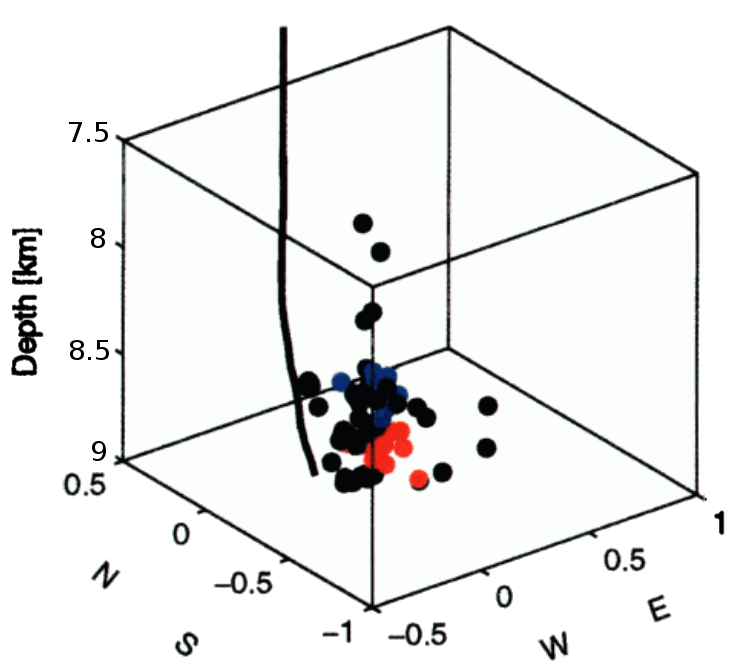
\includegraphics[scale=0.11]{img/KTB1994_hypocenters_3D.png}}
    \end{itemize}
        {\tiny Source: Zoback and Harjes, 1997}
    \pause
  \item \textbf{KTB2000}: $4000\physu{m^3}$ of fresh water
    \begin{itemize}
     \item Pumped into the hole encasing
         \pause
          \fromtopline{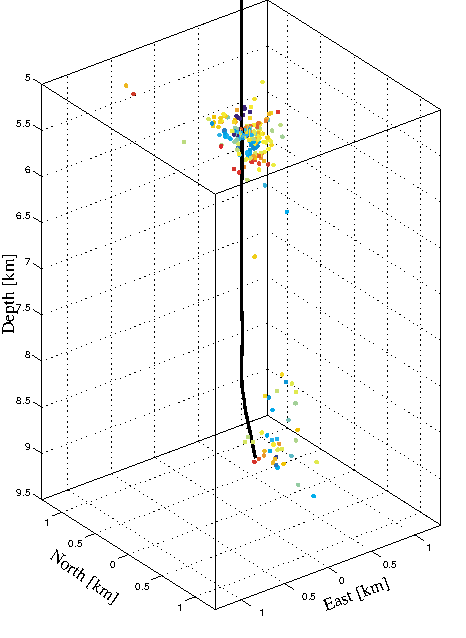
\includegraphics[scale=0.4]{img/KTB2000_hypocenters_3D.pdf}}
    \end{itemize}
 %   {\tiny Source: Baisch et. al 2002}
 \end{itemize}
\end{frame}

\begin{frame}{KTB2000 injection}
 \begin{itemize}
  \item 21 August -- 19 October 2000 
    \pause
  \item Stepwise increased flow rate
 % 30 l/min at begin, 70 at end
   \\ 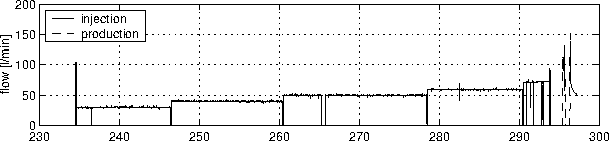
\includegraphics[scale=0.87]{img/KTB2000_flowrate.pdf}
  \item<4->
    \fromtopline{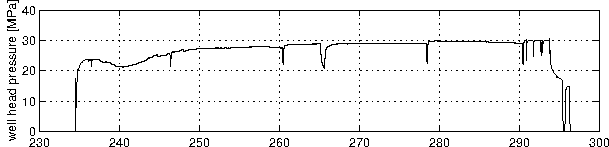
\includegraphics[scale=0.87]{img/KTB2000_pressure.pdf}}
 % pressure 300 atmospheres
 % power 35 kW
  \item<3->
    \fromtopline{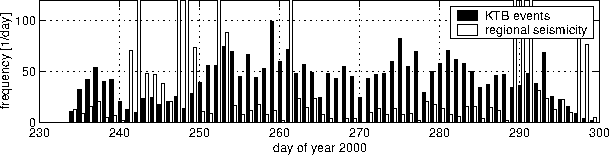
\includegraphics[scale=0.87]{img/KTB2000_eventrate.pdf}}
 \end{itemize}
\end{frame}

\begin{frame}{Seismic network}
 \begin{itemize}
  \item Sonde in pilot hole
    % 3-component, 1 kHz
    \pause
  \item Network of 40 surface stations
    \pause
   \\ 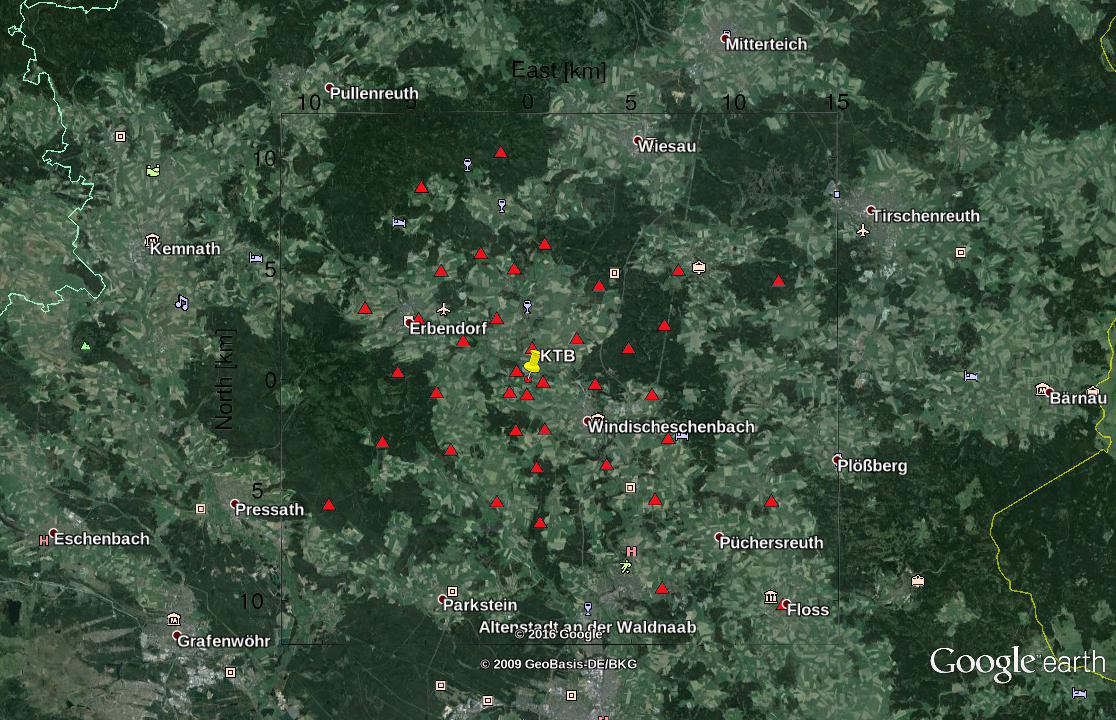
\includegraphics[scale=0.34]{img/SeismicNet-GE.png}
 \end{itemize}
\end{frame}

\begin{frame}{Location determination}
    \pause
 \begin{itemize}
  \item P-S arrival time difference
   \\ 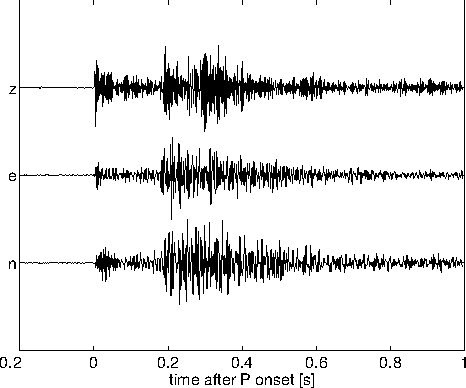
\includegraphics[scale=1]{img/PilotSonde_rawData.pdf}
 \end{itemize}
\end{frame}

\begin{frame}{Location determination}
 \begin{itemize}
  \item P-S arrival time difference
   \\ 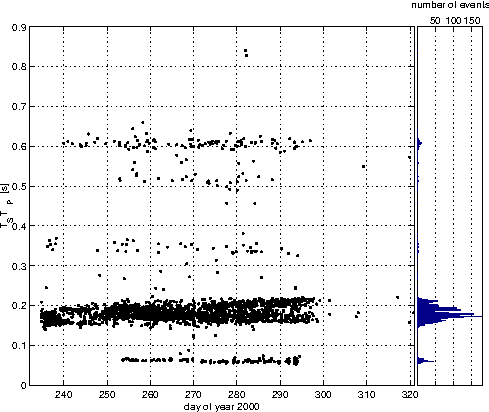
\includegraphics[scale=1]{img/PilotSonde_eventHisto.pdf}
 \end{itemize}
\end{frame}

\begin{frame}{Location determination}
  \begin{center}
    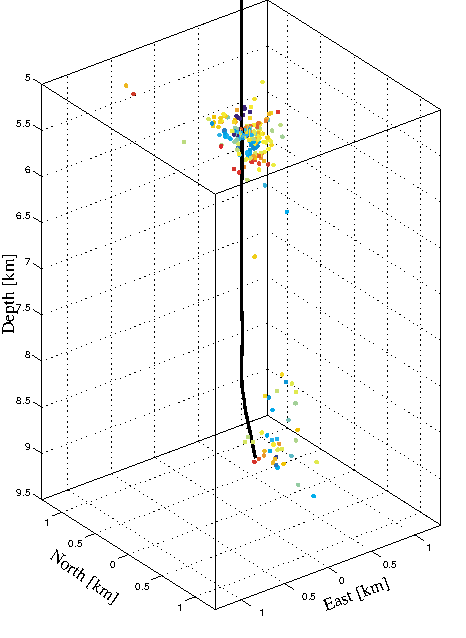
\includegraphics[scale=0.7]{img/KTB2000_hypocenters_3D.pdf}
  \end{center}
\end{frame}

\end{document}

